To evaluate effectiveness of the attacks, I trained a classifier for age estimation. 
First I describe the dataset I used to train the classifier and then I present results of training. 

For training data, I created a dataset based on two datasets: the APPA-REAL dataset \cite{agustsson2017appareal}  and the UTK Face dataset \footnote{https://susanqq.github.io/UTKFace/}.

The APPA-REAL dataset contains 7,591 images with associated age labels. The dataset is split into 4113 train, 1500 valid and 1978 test images. For each image in the dataset, there is also the corresponding image which contains the cropped face. Distribution of samples over age for training dataset is presented in Figure \ref{fig:appa-train-stats}.

The UTK Face dataset consists of 23252 images with associated age labels. I preprocessed every image to extract a face\footnote{every face is cropped with 40\% margin} from it. For face detection, I used Dlib \cite{dlib09} library. Distribution of samples over age is presented in Figure \ref{fig:utk-stats}.

In constructed my training dataset as union of all the images from the UTK Face dataset and training images from the APPA-REAL dataset . For my validation dataset and my test dataset I used validation images and test images from the APPA-REAL validation and test dataset, respectively. 

\begin{figure}[h]
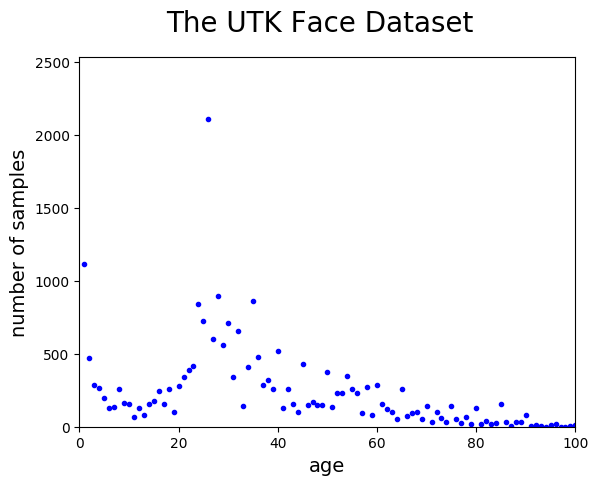
\includegraphics[width=13cm]{utk-stats}
\caption{Number of samples per age in the UTK Face Dataset}
\label{fig:utk-stats}
\end{figure}

\begin{figure}[h]
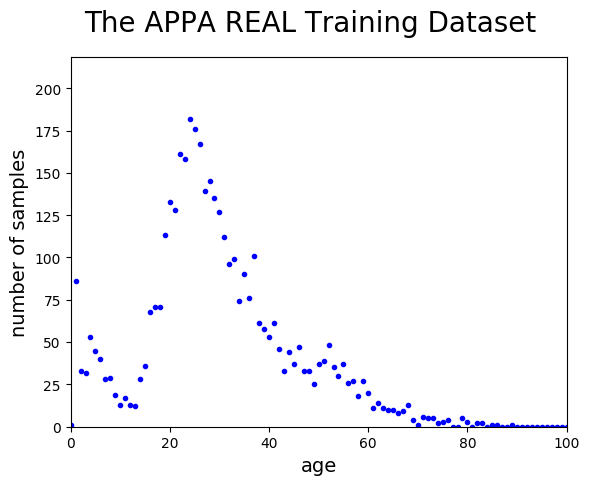
\includegraphics[width=13cm]{appa-train}
\caption{Number of samples per age in the APPA-REAL Training Dataset}
\label{fig:appa-train-stats}
\end{figure}

Instead of training a DNN from scratch, I used a pretrained DNN that is trained on the ImageNet dataset and fine-tuned it for age estimation. In other words, I downloaded already existing model of a DNN and re-trained it for my specific task, i.e. age estimation. This technique is called \textit{transfer learning} and more information about it can be found in \cite{yosinski2014transferable}.

Instead of measuring accuracy of a classifier, in the age estimation domain usually a mean absolute error is measured. If a person who is 65 years old gets classified as 66 years old, a classifier did actually a good job although it didn't predict the correct class. However, if a person who is 65 years old gets classified as 6 years old, that is a significantly bigger mistake than classifying it as 66 years old. Yet, when computing an accuracy, there is no difference if a predicted class is 6 or 66 if a ground truth is 65. That is intuition why mean absolute error is used instead of accuracy as a metric.

When it comes to (targeted) misclassification, there is something in age estimation domain that needs to be taken care of. If a person is classified a year or two older, it is not a huge success for a (targeted) misclassification. In the experiments that follow, targeted version of attacks is used, but a label is set as follows. If a person is under 50 years old, the target label is 90 years old. If a person is 50 years old or older, the target label is 10 years old. 

The idea behind such a setting is to maximize mean average error, i.e. make classificator as wrong as possible, using the targeted version of known attacks.  This is how I reused targeted attacks in a novel setting. Initially I put targeted labels to 0 and 100 instead of 10 and 90, respectively, but I observed a worse performance. Probably because they are on the edge of the considered age range.

Two different optimizers are used in the experiments for minimizing a loss function: SGD, introduced in Section \ref{subsection:gradient-descent}, and Adam \cite{DBLP:journals/corr/KingmaB14}. Two different DNN architectures are used for training: ResNet-50 \cite{DBLP:journals/corr/HeZRS15} and VGG16 \cite{DBLP:journals/corr/SimonyanZ14a}. Their performance is presented in Table \ref{table:trained-models}.

\begin{table}[]
\centering
\begin{tabular}{|c|c|c|c|c|}
\hline
Id & Architecture & Optimizer & Validation Loss & \textbf{Validation MAE} \\ \hline
1 & ResNet-50 & SGD & 3.436 & 5.151 \\ \hline
2 & ResNet-50 & Adam & 3.456 & 6.772 \\ \hline
3 & VGG16 & SGD & 16.603 & 11.255 \\ \hline
4 & VGG16 & Adam & 15.494 & 11.685 \\ \hline
\end{tabular}
\caption{Different models trained}
\label{table:trained-models}
\end{table}

